\documentclass[aspectratio=169]{beamer}

\usepackage[croatian]{babel}
\usepackage[T1]{fontenc}
\usepackage[utf8]{inputenc}
\usepackage{lmodern}
\usepackage{microtype}
\usepackage{csquotes}
\usepackage[natbibapa]{apacite}
\usepackage{url}
\usepackage{fontawesome}
\usepackage{listings}

\definecolor{twitterBlue}{HTML}{1DA1F2}

%%%%% titlepage
\title[]{Rad s tabličnim podacima}

\author[]{\fontsize{8}{10}\selectfont Denis Vlašiček\\[.15em]
    Odsjek za psihologiju FFZG | CROSSDA\\[.15em]
    \faEnvelope\ dvlasice@ffzg.hr\\[.15em]
    \textcolor{twitterBlue}{\faTwitter} @dvlasicek\\[.15em]
    \faGithub\ vdeni}

\titlegraphic{\vspace*{-2em}\includegraphics[scale=.30, keepaspectratio=true]%
    {images/walrus-inspector-sheet.pdf}}

\date[]{}
%%%%%

%%%%% prilagodba referenci na hrvatski
\renewcommand{\BCBT}{}
\renewcommand{\BCBL}{}%  comma before last author when no. of authors > 2
\renewcommand{\BOthers}[1]{i sur.\hbox{}}% ``and others''
\renewcommand{\BBAA}{i}
\renewcommand{\BBAB}{i}
\renewcommand{\BIn}{U:}
\renewcommand{\BED}{Ur.\hbox{}}
\renewcommand{\BEDS}{Ur.\hbox{}}
\renewcommand{\BPGS}{str.\hbox{}}
\renewcommand{\BRetrievedFrom}{Preuzeto s:\hbox{}}
\renewcommand{\BEd}{izdanje}
\renewcommand{\BVOL}{svezak}
%%%%%

\setcounter{tocdepth}{1}

%%%%% beamer tema
\usetheme{CambridgeUS}

\usecolortheme{dove}

\setbeamertemplate{itemize items}[default]

\setbeamertemplate{itemize item}{\textbullet}
\setbeamertemplate{itemize subitem}{\(\triangleright\)}

% \setbeamertemplate{section in toc}%
%     {\inserttocsectionnumber) \inserttocsection}

\setbeamertemplate{section page}{
    \begin{centering}
        \Large
        \insertsection\par
    \end{centering}
}

\setbeameroption{hide notes}
%\setbeameroption{show only notes}
%\usepackage{pgfpages}
%\setbeameroption{show notes on second screen=left}

%%%%%

%%%%% serif font kao default
\usefonttheme{serif}
%%%%%

\setbeamertemplate{navigation symbols}{}

\makeatletter
\newenvironment{noheadline}{
    \setbeamertemplate{headline}{}
}{}
\makeatother
%%%%%

%%%%% nastavljanje enumerate
\newcounter{saveenumi}
\newcommand{\seti}{\setcounter{saveenumi}{\value{enumi}}}
\newcommand{\conti}{\setcounter{enumi}{\value{saveenumi}}}

\resetcounteronoverlays{saveenumi}
%%%%%

%%%% fontsize za bibliografiju
\renewcommand*{\bibfont}{\scriptsize}
%%%%%

%%%%% tiny citep
\newcommand{\tinycitep}[1]{%
    \bgroup
    \scriptsize
    \citep{#1}
    \egroup}
%%%%%

%%%% listings
\lstset{basicstyle=\footnotesize\ttfamily}

\begin{document}

\begin{frame}
    \titlepage
\end{frame}

\section{Uvod}

\begin{noheadline}
    \begin{frame}
        \sectionpage
    \end{frame}
\end{noheadline}

\begin{noheadline}
    \begin{frame}
        \frametitle{Uvod}

        \leavevmode

        \makebox(0, 0){%
        \put(10, 50){
\includegraphics[scale=.40]{images/excel-at-covid.png}}}

        \pause

        \makebox(0, 0){%
        \put(90, 0){
\includegraphics[scale=.40]{images/rename-genes.png}}}

    \end{frame}
\end{noheadline}

\section{Kako se obraniti od ružnih podataka?}

\begin{noheadline}
    \begin{frame}
        \sectionpage

        \begin{center}
            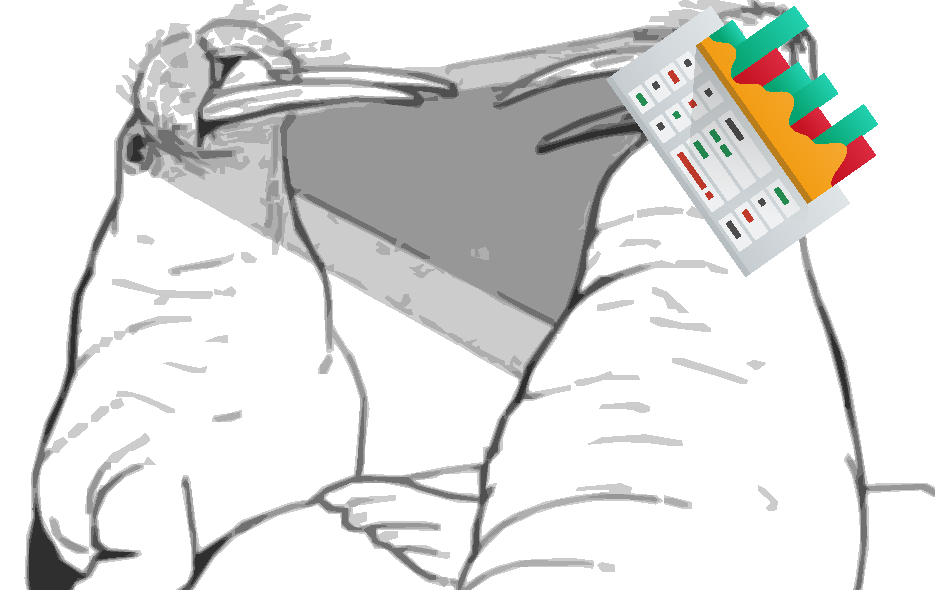
\includegraphics[scale=.35]{images/walrus-combat-sheet.pdf}
        \end{center}
    \end{frame}
\end{noheadline}

\begin{noheadline}
    \begin{frame}
        \frametitle{Kako se obraniti od ružnih podataka?}

        \begin{columns}

            \column{.50\linewidth}

            \begin{itemize}
                \setlength{\itemsep}{2em}

                \item što god radili, budite konzistentni

                \vspace{1em}
                
                \pause

                    \begin{itemize}

                        \setlength{\itemsep}{2em}

                        \item konzistentna imena varijabli

                        \item konzistentne oznake vrijednosti

                        \item konzistentna imena datoteka

                        \item konzistentan format datuma

                    \end{itemize}
            \end{itemize}

            \pause

            \column{.50\linewidth}

            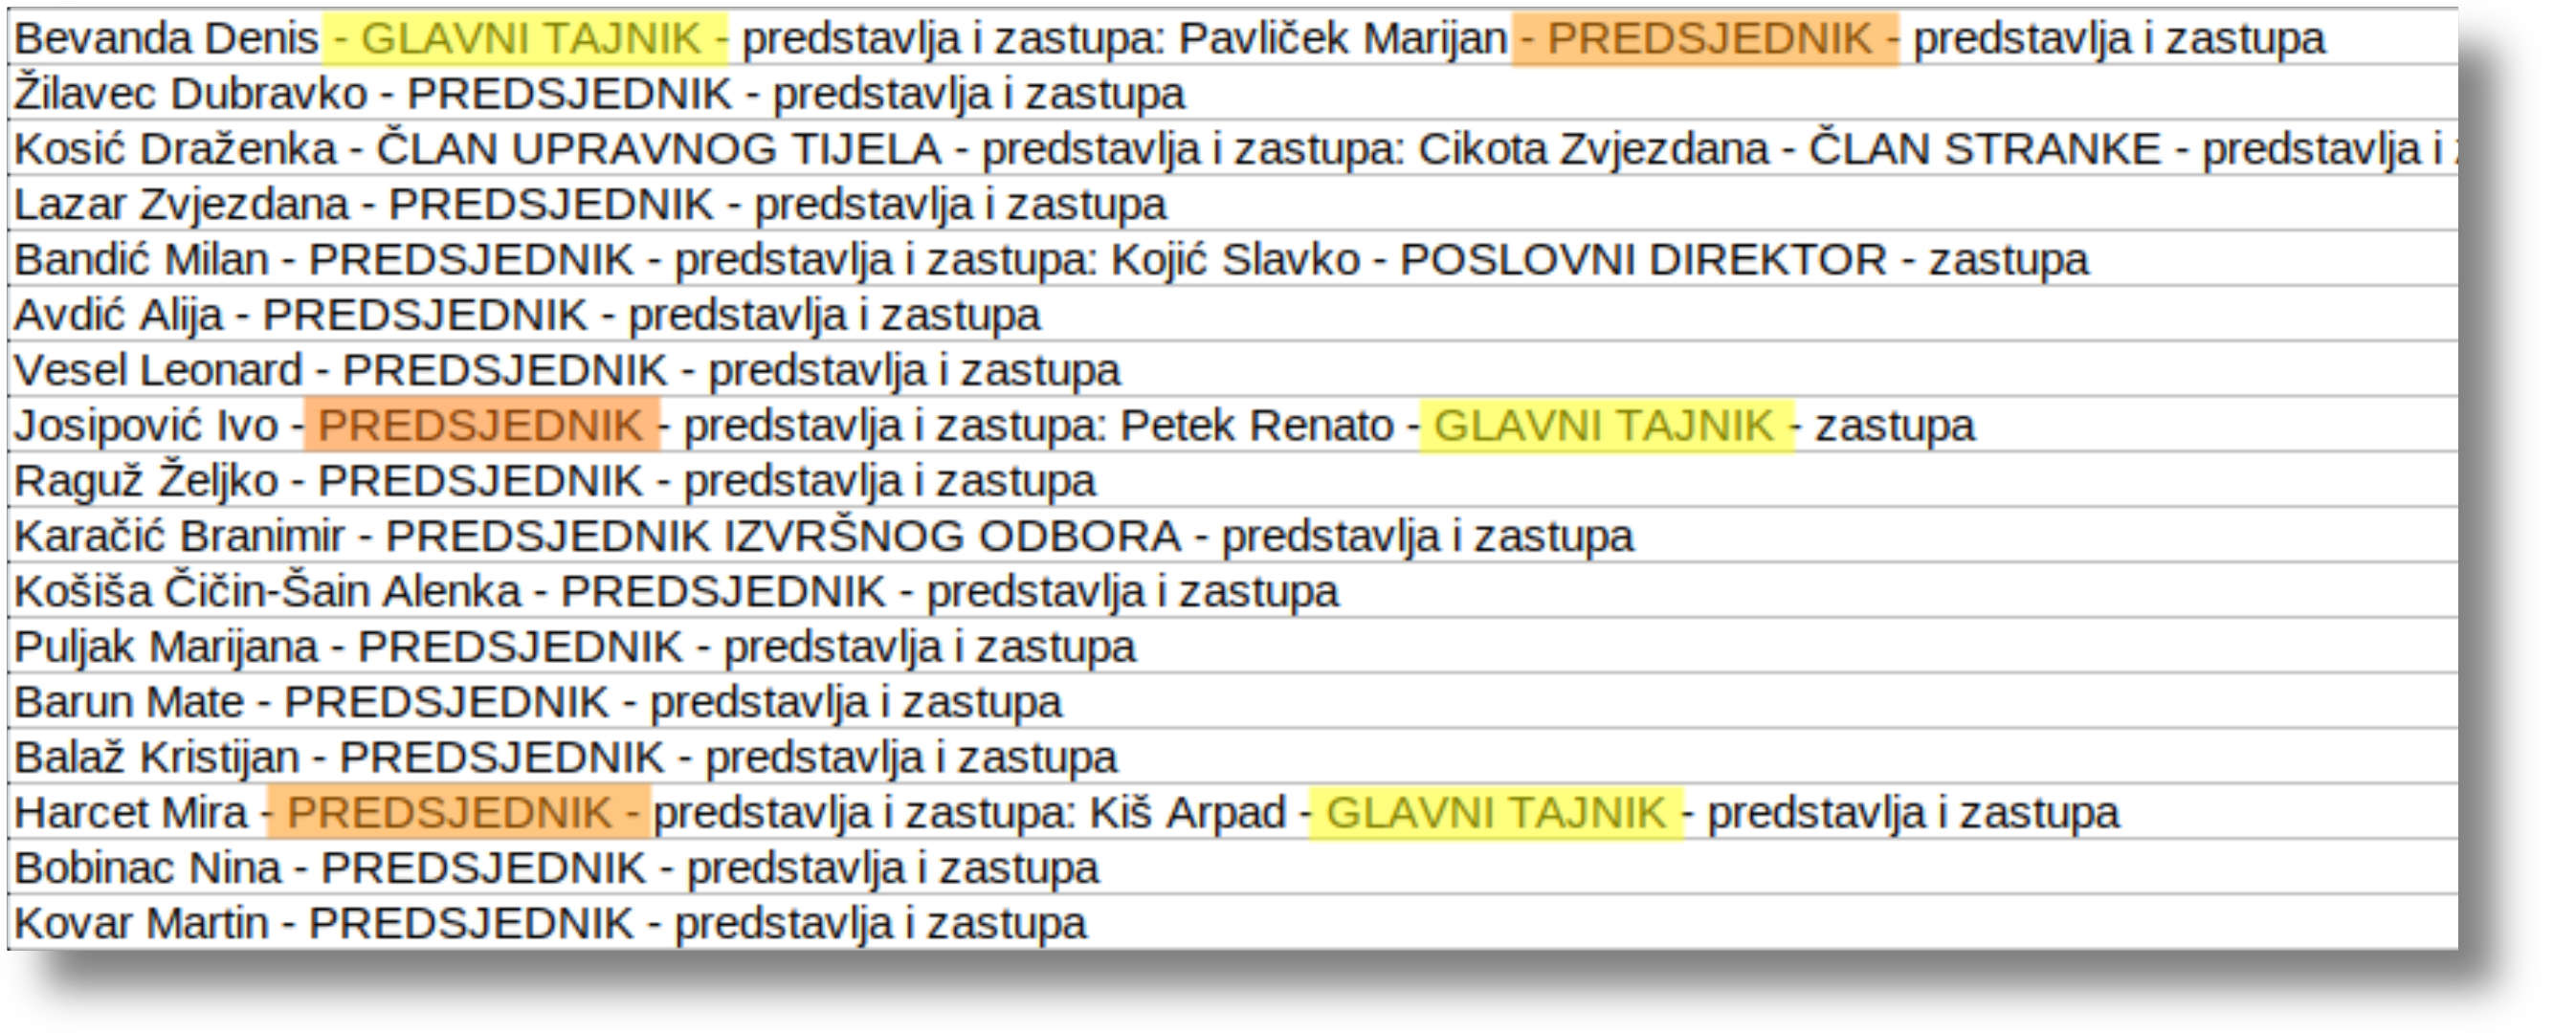
\includegraphics[scale=.30]{images/konzistentan-predsjednik.png}

        \end{columns}
    \end{frame}
\end{noheadline}

\end{document}
